% paper=a4paper (default),letterpaper,a5paper,b5paper,executivepaper,legalpaper
% font=
% fontsize=10pt, 11pt, 12pt (10pt por defecto)
% documentclass=article,report,book,letter,"ieeetran"
% draft=draft (no carga imagenes, pero indica lugares)
% columns=onecolumn(default), twocolumn
% margenes=oneside,twoside
\documentclass[a4paper,12pt]{article}

%\usepackage[options]{paquete}
\usepackage[spanish]{babel}
\usepackage[utf8]{inputenc}
\usepackage[T1]{fontenc}
\usepackage{graphicx}
\usepackage{amsmath}

\title{Portada base en LaTeX}
\date{\today}
\author{Martin Casatti}

\usepackage{lipsum}

\begin{document}
	\maketitle
	\begin{abstract}
		\lipsum[1-2]
	\end{abstract}
	%\clearpage

	Hola mundo!
	
	un texto que contiene un montón de ñoñadas en español.
	
	\lipsum[1-1]

%	\chapter{Capitulo numerado}
%%	\lipsum[1-2]
%	\section{Seccion numerada}
%	
%	\section{Otra}
%%	\lipsum[1-1]
%	\subsection{Subseccion numerada}
%%	\lipsum[1-1]
%	\subsubsection{Subsubseccion numerada}
%%	\lipsum[1-1]
%	\paragraph{Parrafo}
%
%	\subparagraph{Subparrafo}
%
%%	
%	\chapter*{Capitulo no numerado}
%%	\lipsum[1-2]
%	\section*{Seccion no numerada}
%%	\lipsum[1-1]
%
%	\begin{itemize}
%		\item Un contenido extremadamente largo para que sirva de ejemplo
%		\item Dos
%		\item Tres
%		\begin{itemize}
%			\item Tres Uno
%			\item Tres Dos
%		\end{itemize}
%	\end{itemize}
%%
%	\begin{enumerate}
%		\item Uno
%		\item Dos
%		\begin{enumerate}
%			\item Anidado
%		\end{enumerate}
%		\begin{itemize}
%			\item Viñeta
%			\item Otra viñeta
%		\end{itemize}
%		\item Cuatro
%	\end{enumerate}
%%
%	\begin{description}
%		\item[Etiqueta] Descripcion
%		\item[RDBMS] Sistema de administracion de bases de datos
%	\end{description}

	\begin{figure}[h]
		\centering
		
\includegraphics[]{tech1}
		\caption{Tecnologia}
		\label{fig:tecnologia}
	\end{figure}

	Este es un texto que referencia la figura \ref{fig:tecnologia} para que veamos como funcionan los contadores.

	\begin{table}[h]
		\centering
		\begin{tabular}{|l|r|}
			\hline
			Celda solitaria & \\
			\hline
			Columna 1 & Columna 2\\
			\hline
			Otra fila con mas texto & Otra columna\\
			\hline
		\end{tabular}
		\caption{Una tabla}
		\label{tab:una-tabla}	
	\end{table}

Este es un texto referenciando una tabla (numero \ref{tab:una-tabla}) para ver como funciona
% Matemáticas
	
Formula inline $f(x) = x^2$ embebida en el texto.	


	\begin{equation*}
		g(x) = \frac{x^2}{\sqrt{x^{(2+i)}}} 
	\end{equation*}
%
	\begin{align*}
		1 + 2 &= 3\\
		1 &= 3 - 2\\
		-2 + 3 &= (1+1+1) - 2
	\end{align*}
	
	$
	\left[	
	\begin{matrix}
		1 & 0\\
		0 & 1
	\end{matrix}
	\right]
	$
	
	%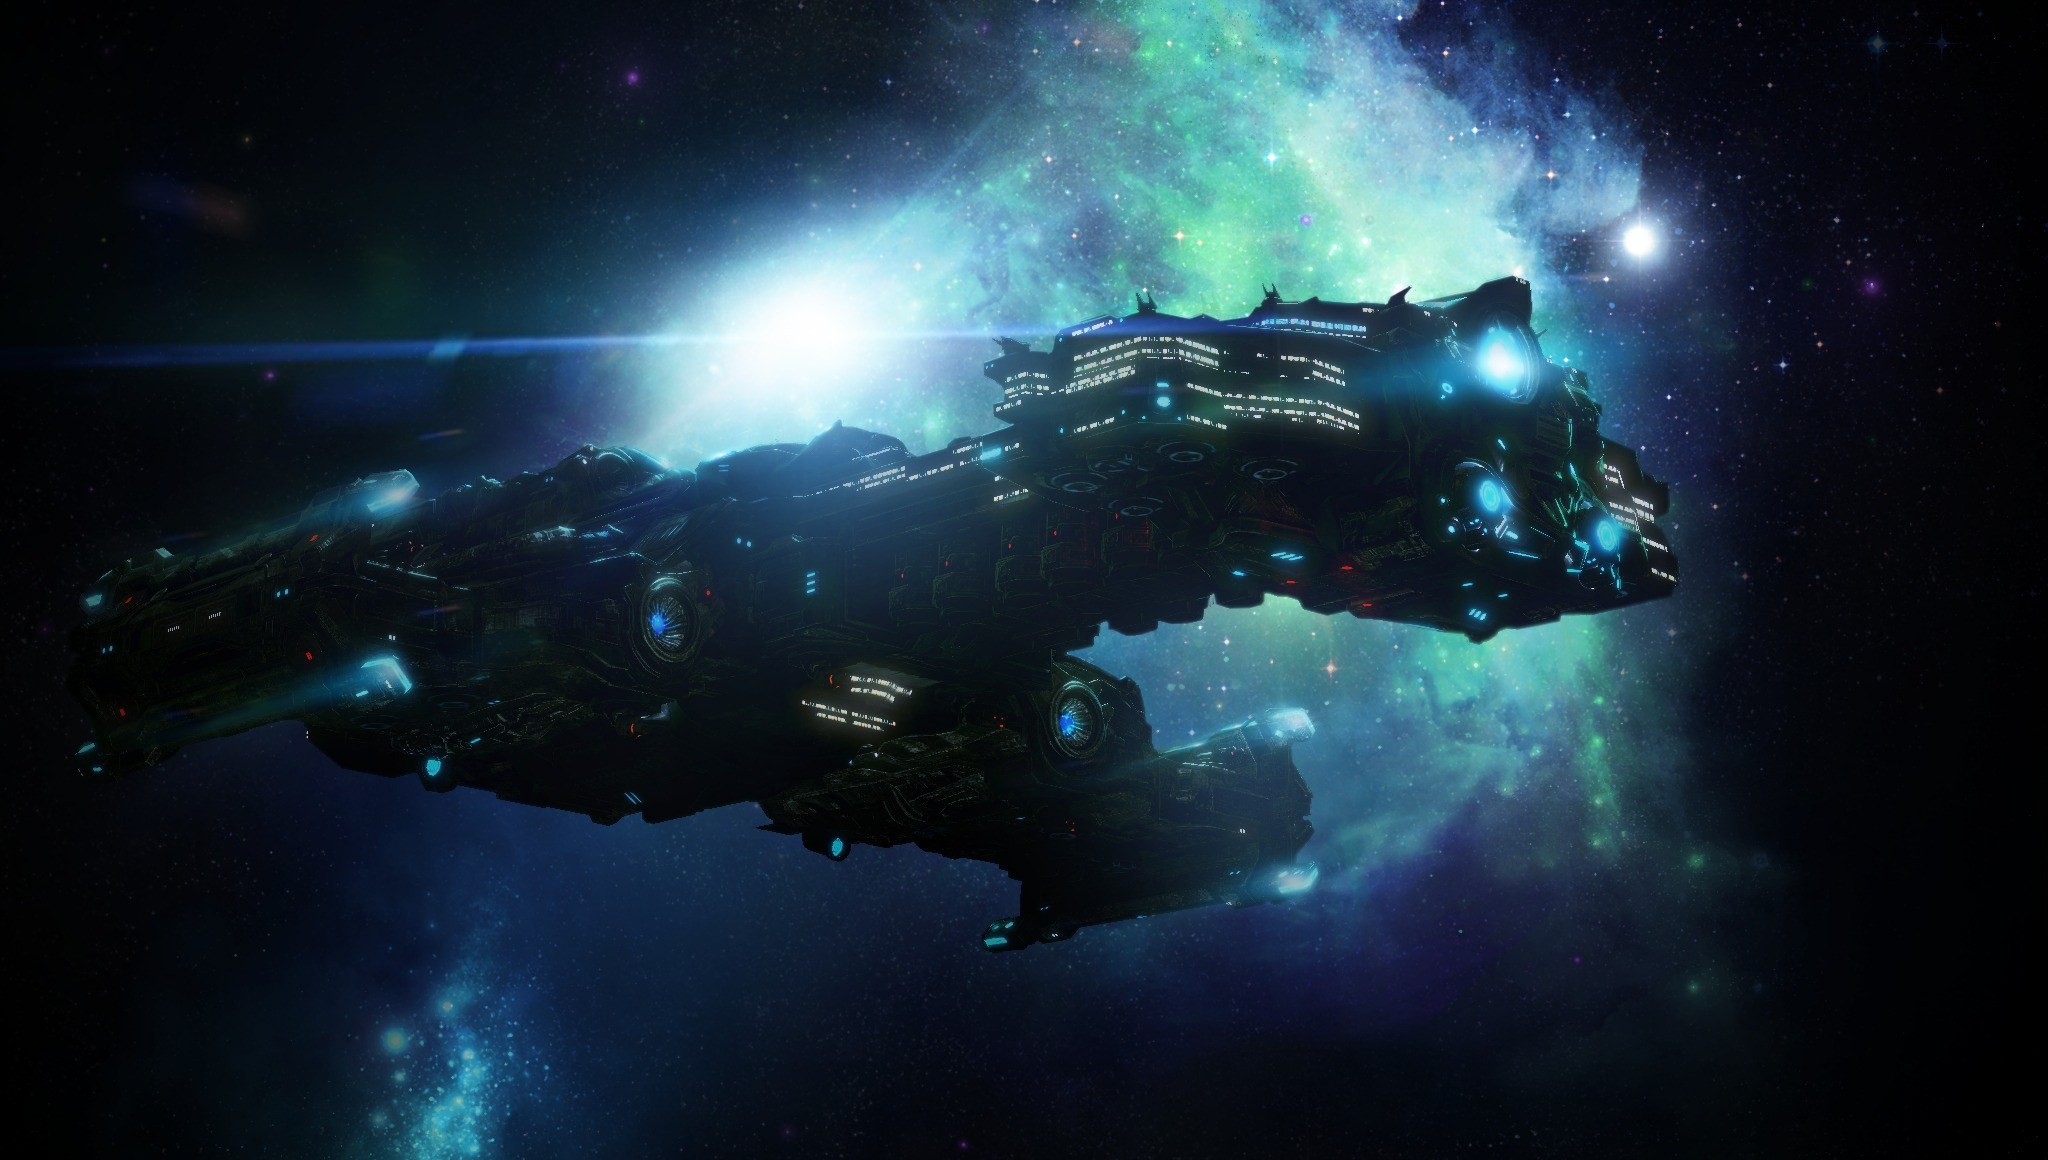
\includegraphics[scale=0.1]{ship1}
	%
\includegraphics[width=250px]{tech1}
	
\end{document}